\pdfoutput=1

\documentclass{l4proj}

%
% put any packages here
%
\usepackage{graphicx}
\graphicspath{ {images/} }

\begin{document}
\title{Source Code Clippy (Scclippy) - IDE Micro-Task Recommender Plugin}
\author{Boris Nikolov}
\date{2015/2016}
\maketitle

\begin{abstract}
The Source Code Clippy plugin enables searching for code snippets from different sources and provides them to the developer. 
SHOULD DIFFERENT WAYS OF SEARCHING BE EXPLAINED? @@@@@@@@@@@@@@@@
The main objective of the project is to build a plugin for an IDE that will support the user with searching and helpful related features, as well as giving them the ability to configure the system. There is a research interest in how beneficial excerpts of code are to the developers. Thus, the application's purpose is to provide tools with which the user can easily and intuitively interact. 
The system has been evaluated ... . The findings of the study show that ... . Feedback from users ... . Besides personal purposes, the plugin can be used ... ??? @@@@@@@@@@@@@@@@
\end{abstract}

\educationalconsent
%
%NOTE: if you include the educationalconsent (above) and your project is graded an A then
%      it may be entered in the CS Hall of Fame
%
\tableofcontents
%==============================================================================

\chapter{Introduction}
\pagenumbering{arabic}

\section{Project context}

We have recently begun to explore a new area of research on micro-scale or end user software engineering. The goal of this project is to address the needs of end user software developers who are engaged in short term micro scale software development projects. Examples include the development of a script to configure an Arduino project; an excel macro for processing a spreadsheet of data or a python script to batch process a large number of pictures. Existing software engineering tools are not suitable for these projects because they are generally targeted at long term large scale efforts and require a considerable upfront investment. 

Various recommendation systems designed for software engineering purposes have been becoming more popular in recent years. Their purpose is to assist developers of all skills to find the information they need. This project is about building a tool that can help users to see usages of similar code by suggesting excerpts of code.

\section{Motivation}

The motivation for this project is to gain understanding of how useful code snippets are to developers. In addition, there are not many applications that provide searching for excerpts by retrieving data from different sources inside an IDE (Integrated Development Environment). This provides a chance to build such system, which will give the user the ability to choose between multiple options and be configured according to their preferences.

\section{Objectives}

A prototype code snippet recommender system for Sublime was developed by Tomasz Sadowski. This prototype continually monitors the contents of a developer's editor and searches Stack Overflow for similar snippets of code using an information retrieval engine (Terrier is used in the prototype). For example, a developer is working on a script to process text files and has started on the task of opening files. The recommender tool searches for relevant code snippets on Stack Overflow and presents them for auto insertion into the editor.

The goal of this project is to re-develop the prototype as a production quality plugin for an Integrated Development Environment such as Eclipse, IntelliJ, Visual Studio, Emacs or PyCharm. The plugin will help developers achieve small tasks and therefore should be highly usable so that the user can do their work seamlessly. In addition, the scope of the recommender's input should also be controllable, so that recommendations can be made on the basis of the currently typed command, or a selected range of text.

\section{Achievements}

The required plugin Source Code Clippy was successfully implemented as an IntelliJ IDE plugin for the Java programming language. It allows the user to search for code snippets in four different ways - by making requests to Stack Exchange excerpts API; by indexing files on disk; using a Web Service that has already indexed a collection of Stack Overflow documents; by performing Google search on the query. The plugin also offers useful to the user features - searching for code is done automatically when the user is typing as well as when the user selects part of their code; automatic insertion of code into the editor by double clicking on post and others.  
In terms of qualities, the plugin could be described as highly usable, efficient, customizable, and extensible.

\section{Dissertation structure}
The dissertation is structured in a chronological order. It starts with the background and requirements, follows the design and implementation process, and ends with the results of the evaluation and a discussion on the outcome of the project. The table below describes the report's structure.

\begin{table}[h]
\caption{Dissertation Structure}
\centering
\def\arraystretch{1.5}
\begin{tabular}{p{3cm}p{12cm}}
\hline
Chapter & Content \\
\hline
2. Background  & A short description of the previous work related to the project. \\
3. Requirements   & Discusses the gathering of the requirements, followed by a list of all requirements. \\
4. Design and Implementation  & Describes the architecture of the plugin. Details the design decisions taken. Also contains a list of final design features.\\
5. Evaluation  & Describes the test process and the user evaluation carried out, their results and a discussion of the results. \\
6. Conclusion: & Discusses the outcome of the project, future work possibilities and learning outcomes.  \\
\hline
\end{tabular}
\label{table:reportStructure}
\end{table}


\section{Terminology}
SCC refers to the Source Code Clippy (SCClippy) plugin.
\\
\\
RSSE is an abbreviation for Recommendation Systems for Software Engineering.

\chapter{Background and Requirements}

\section{Related work}

In the previous years, a number of recommendation systems for Software Engineering have been developed to help developers with information and evaluation of alternative decisions. Most such systems have been focused on assisting while the users are in the process of programming.

\subsection{Similar technologies}

INCLUDE REFERENCES @@@@@@@@@@@@@@@@

There are many RSSE systems that use different input, as well as processing and visualisation techniques. Similar plugins have been outlined below:

The Eclipse IDE plugin eRose mines data from repositories such as Concurrent Versions System (CVS). It tracks consecutive changes in code and makes suggestions based on that information. The data is displayed in a separate view, after each save operation.

Another example is the Strathcona system which extracts data about the structure of a code fragment in order to search a PostgreSQL database and use heuristics to rank the results. It shows a structural overview, as well as highlights based on the difference from the user's code. This system is particularly useful for frameworks that have been poorly documented.

Suade is also an Eclipse plugin which is specialised in automatically presenting suggestions by retrieving related elements (fields, methods). By design, it contains a dependency graph of the elements that can be interactively and iteratively updated by the developer.

CodeBroker uses as input the comments written by developers to assist them. A recommendation is produced every time a comment is written by analyzing the text and doing type-signature matching. The system also manages user-specific lists.

Dhruv is a system that recommends people and artifacts based on bug reports. It extracts data from the open source community (different types of users and content and their interactions) to create a Semantic Web, which later is used to match that to the bug report's information.

Expertise Browser recommends people for a particular piece of code by considering the people who have modified the content in the past. However, an assumption is made that whoever made changes beforehand is an expert.

ParseWeb is useful in situations when the developer needs an object to perform methods on, but cannot recall how to get the object. The tool crawls the web based on the user's input (object types) to search for recommendations.

\subsection{Evaluation of similar ideas}
Most systems and tools described above have something in common - they do recommendation by going through several stages - input handling, intermediate analyzing of some sort, and visualisation technique. However, they also have a unique approach that focuses on certain aspects. Source Code Clippy is special because it features different ways of searching for excerpts by focusing on getting data from Stack Overflow - one of the biggest sources of code snippets. In addition, the plugin offers helpful features to assist the developer.


\section{Description of Tomasz's prototype}
The Source Code Clippy plugin is a continuation of an already build prototype for Sublime which Tomasz Sadowski developed. The prototype has a single feature that enables the user use the developer's editor and search Stack Overflow for similar snippets of code using an information retrieval engine (Terrier is used in the prototype). 

For example, a developer could be working on a script to process text files and has started on the task of opening files. The recommender tool searches for relevant code snippets on Stack Overflow and presents them for auto insertion into the editor. 

The prototype was not evaluated.

\section{Requirements Elicitation and Gathering}
Requirements were gathered and discussed during informal weekly customer meetings.
The requirements and tasks were prioritised based on the MoSCoW approach (link). Github's issue tracker was used to list all of them and track their progress. (https://github.com/thrios/SourceCodeClippy/issues)

\subsection{Must Have}
Must have requirements are fundamental and crucial to the success of the project. Table ~\ref{table:mustTable} shows the details of the must-have requirements.

\begin{table}[h]
\caption{Must Have Requirements}
\centering
\def\arraystretch{1.5}
\begin{tabular}{p{2cm}p{4cm}p{9cm}}
\hline

FR & Requirement & Description \\
\hline
1 & Searching with local index & Based on some input, the user must be able to search using an index on the local file system, as well as create a new index/update existing one.\\
2 & Searching with Stack Exchange API & The user must be allowed to make requests to the Stack Exchange API based on a query and see the results returned\\
3 & Searching using a Web Service & The user must have the option to choose to search using a web service - a preindexed collection of Stack Overflow question and answer posts\\
4 & Searching with Google for the Stack Overflow domain & The user must be given the option to choose to search the text in the query pane with google\\
5 & Configuration panel & The user must be provided with the functionality to change the settings of the plugin in order to configure and customize it to their needs - changing the local index used, the web service URI, etc\\
6 & Handling selection input & The user's mouse selection should be automatically\\
7 & Last statement typed query input & The user's key input should be captured and update the query input pane\\
\hline
\end{tabular}
\label{table:mustTable}
\end{table}

\subsection{Should Have}
The should have requirements are considered as important. Table ~\ref{table:shouldTable} represents all the 'should have' requirements along with their description.

\begin{table}[h]
\caption{Should Have Requirements}
\centering
\def\arraystretch{1.5}
\begin{tabular}{p{2cm}p{4cm}p{9cm}}
\hline
FR & Requirement & Description \\
\hline
8 & Insertion of code by double clicking a post & A user should be able to login with their Facebook account \\
9 & Filters of results & A user should be able to review the content before uploading, to delete any content that they do not wish to upload \\
10 & Feedback tab & The goal is to improve the system and therefore the user should be able to submit feedback \\
11 & Post useful meta data and customization & Posts should contain their type (question or answer), their score (if applicable) and a hyperlink leading to their source. There should be options to customize the post - let the user choose the text colour used, etc.\\
12 & Custom input pane listener & The user should be able to make search request on 'Enter' and new lines with the 'Shift' key when the focus is on the query pane\\
13 & Additional search request & The plugin should offer an additional search request to be made on the same query to allow more posts to be fetched and displayed\\
14 & Sorting results & The user should be able to sort results by relevance or by score\\
\end{tabular}
\label{table:shouldTable}
\end{table}

\subsection{Could Have}
Could have requirements are optional features the system could benefit from. Due to time constraints, FR21 was not implemented, but is considered for possible future work. Table ~\ref{table:couldTable}  lists the 'could have' requirements, as well as their descriptions.

\begin{table}[h]
\caption{Could Have Requirements}
\centering
\def\arraystretch{1.5}
\begin{tabular}{p{2cm}p{4cm}p{9cm}}
\hline
FR & Requirement & Description \\
\hline
15 & Number of calls to Stack Exchange API & The plugin could display the remaining calls that can be made to the API\\
16 & Highlighting code & Highlighting the text in HTML code tags to distinguish between code and text of a post\\
17 & Write a question & Functionality to enable the user to write a question on Stack Overflow\\
18 & Information tab & A tab for showing information to the user that they might need to know\\
19 & Default number of posts and max number of posts & Feature which gives the user the ability to change how many post they see after a search (on 'Enter'), and a secondary search (using the scroll)\\
20 & Saved settings & The options the user selects and changes could be saved automatically and loaded when the plugin starts\\
21 & Code Intelligent Search & The variable names and other terms in the query that are less relevant could have less weight attributed to them so that the results are more refined. The use of tags that allow the user to filter could be also a potential improvement.\\
\hline
\end{tabular}
\label{table:couldTable}
\end{table}

- A lot of other helpful features such as insertion of code + formatting on double click (instead of standard copy-paste), additional search request on scrolling down; search history; output filters; query input listener; additional data included in posts; notifications; write a question button; provide feedback tab;

In terms of non-functional requirements, the system should have:

\section{Non-Functional Requirements}
Non-functional requirements represent the qualities the system is required to meet. Table ~\ref{table:nonFuncTable}  lists and describes the non-functional requirements for the plugin.
\begin{table}[h]
\caption{Non-Functional Requirements}
\centering
\def\arraystretch{1.5}
\begin{tabular}{p{2cm}p{4cm}p{9cm}}
\hline
NFR & Requirement & Description \\
\hline
1 & Intuitive interface & Users should not get confused and feel the plugin as something they are familiar with \\
2 & High responsiveness/performance in general & The user should not have to wait more than a few seconds \\
3 & High usability & Good user interface, good responsiveness, but also provide helpful features e.g. automating the process if possible and reasonable to do so \\
4 & Good documentation & Well-documented code allows for easy extension of the plugin \\
5 & Extensible & The system should allow for easy future extensions\\
\hline
\end{tabular}
\label{table:nonFuncTable}
\end{table}

\chapter{Design and Implementation}

\begin{figure}[h]
\caption{Architecture diagram}
\includegraphics[scale=0.5]{scc-architecture}
\centering
\label{fig:architecture}
\end{figure}
As you can see in the figure \ref{fig:architecture}, the logical parts of the system are coloured in red. The data sources can be identified by their green colour. The boxes in blue represent outgoing links.

The user can use the IntelliJ SCClippy plugin to retrieve excerpts data from a number of data sources:

- by using a local index on the user's file system. The user is allowed also to create a new index or update the contents of existing one. 

- by sending requests to the Web Service which in return will return a JSON response

- by using the Stack Exchange API to make the request.

- by clicking on a button that will open a browser window and search the query using Google for the domain of Stack Overflow. 

The system also has a hyperlink to an online survey that the user can follow, fill and submit online. The client automatically saves its settings to a file relative to the plugin's installation in order to load them when a new IntelliJ client is started and the plugin was launched. Each instance of IntelliJ contains a separate instance of the SCClippy plugin.

\section{Iterations}
\subsection{Overview}
Consecutive iterations of developing the plugin consisted of several stages:

- Familiarisation with developing a plugin, indexing, and extracting data from the given PostgreSQL database

The process of extracting files from the initially provided database consists of the following steps:\\
1. Writing a query for retrieving questions and another one for answers, both of which add extra empty column for record separation.\\
2. Exporting the results to a csv file with a unique separator\\
3. Using a custom written CSV splitter to create the files used for indexing purposes

- Building an initial version of the plugin that uses a local index, as well as Stack Exchange API search

- Improving the plugin by developing the web service mentioned, automating existing features (input on selection and typing, copying code into editor, etc) and implementing new features such as adding configuration settings, search history, additional search options, feedback and information tabs.

- User Evaluation

\subsection{User Interface}
The user interface was changed frequently in order to keep up with the dynamic requirements and new features each iteration, but also due to ideas about improvements to make the look and feel of the plugin better.

Initial sketches

Basic user interface design

Intermediate design

Final design
\begin{figure}[h]
\caption{Search tab, Darcula IntelliJ theme}
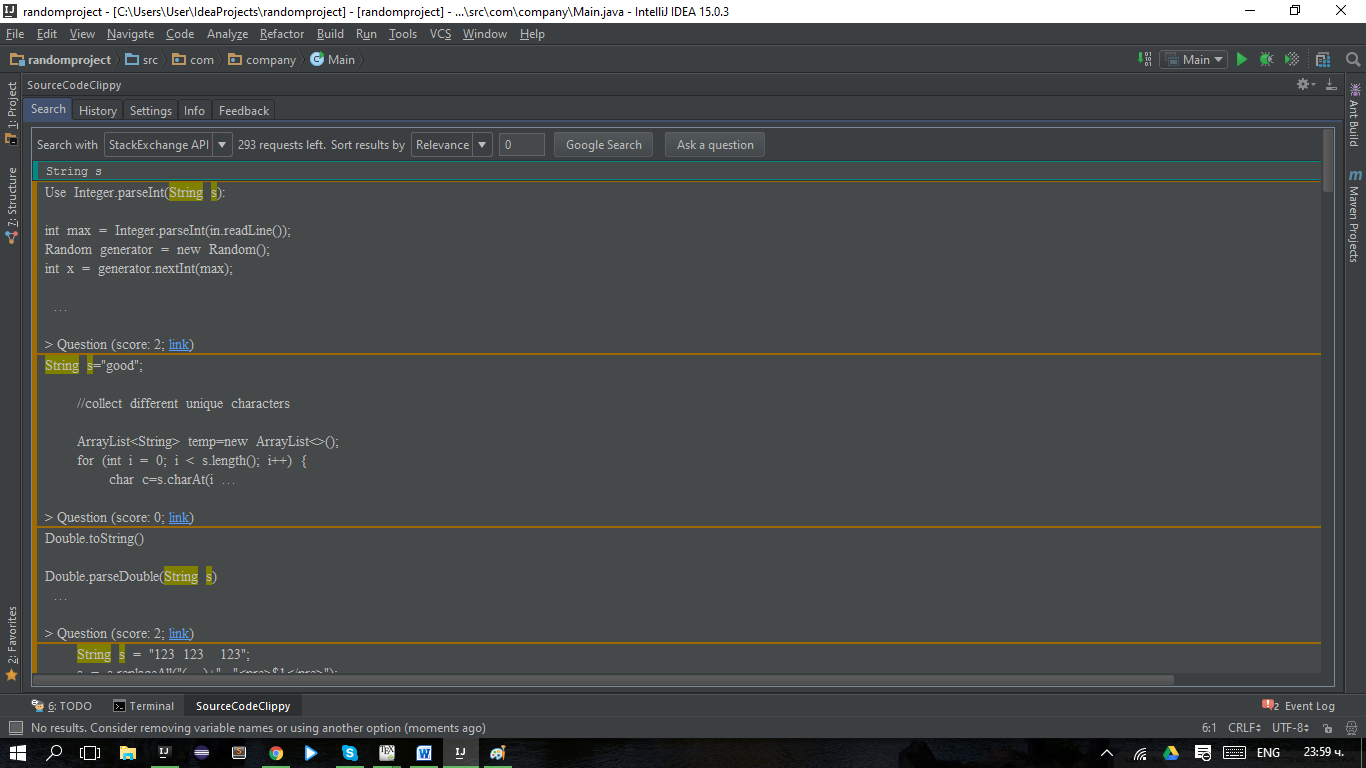
\includegraphics[scale=0.2]{tab-search}
\centering
\label{fig:search-tab}
\end{figure}

\begin{figure}[h]
\caption{Search history tab, Darcula IntelliJ theme}
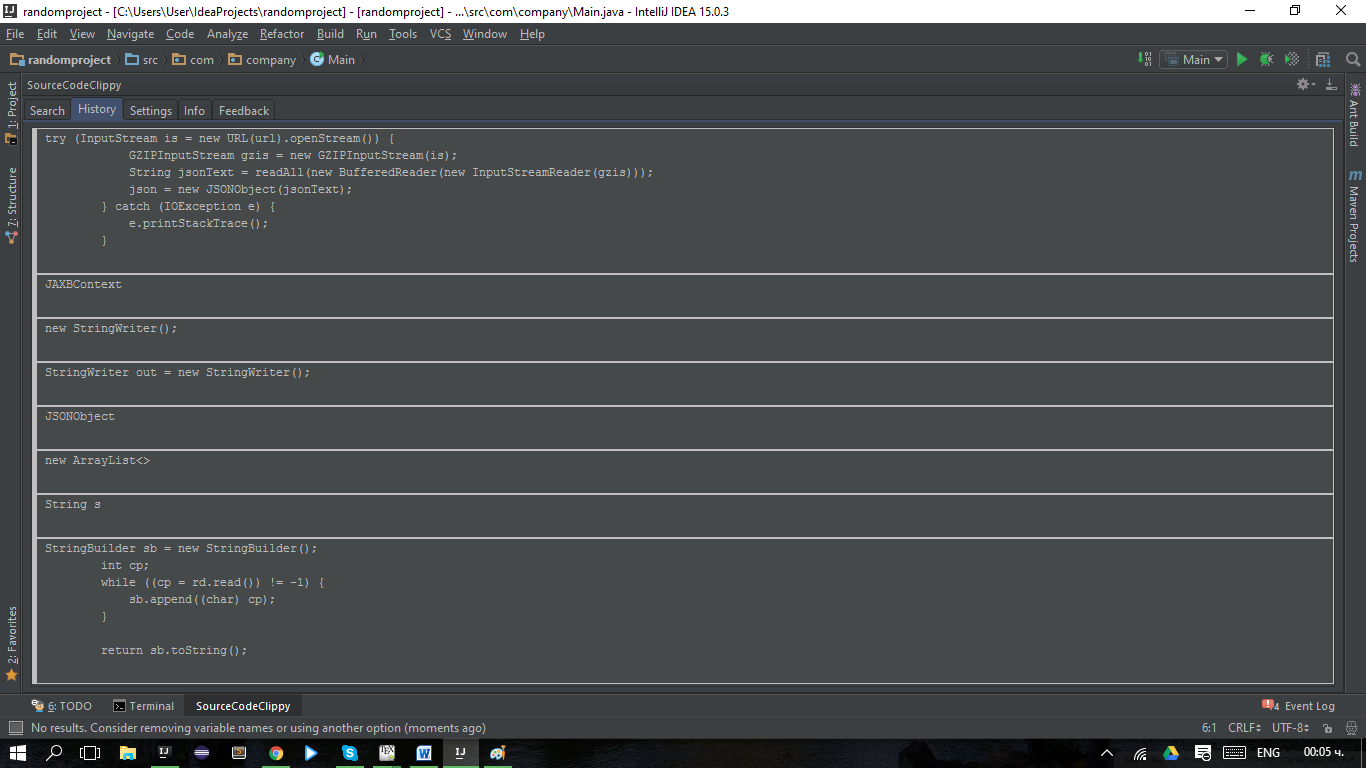
\includegraphics[scale=0.2]{tab-history}
\centering
\label{fig:history-tab}
\end{figure}

\begin{figure}[h]
\caption{Settings tab, Darcula IntelliJ theme}
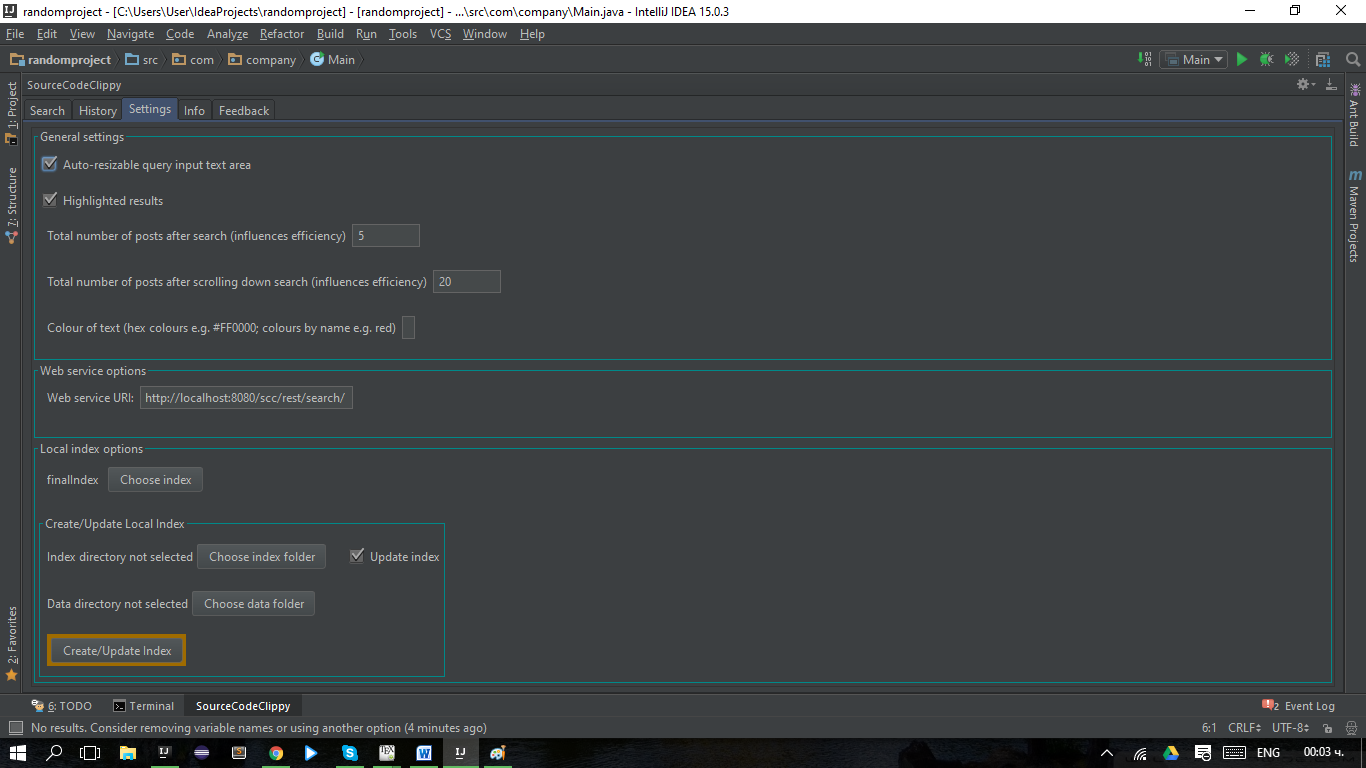
\includegraphics[scale=0.2]{tab-settings}
\centering
\label{fig:settings-tab}
\end{figure}

\begin{figure}[h]
\caption{Information tab, Darcula IntelliJ theme}
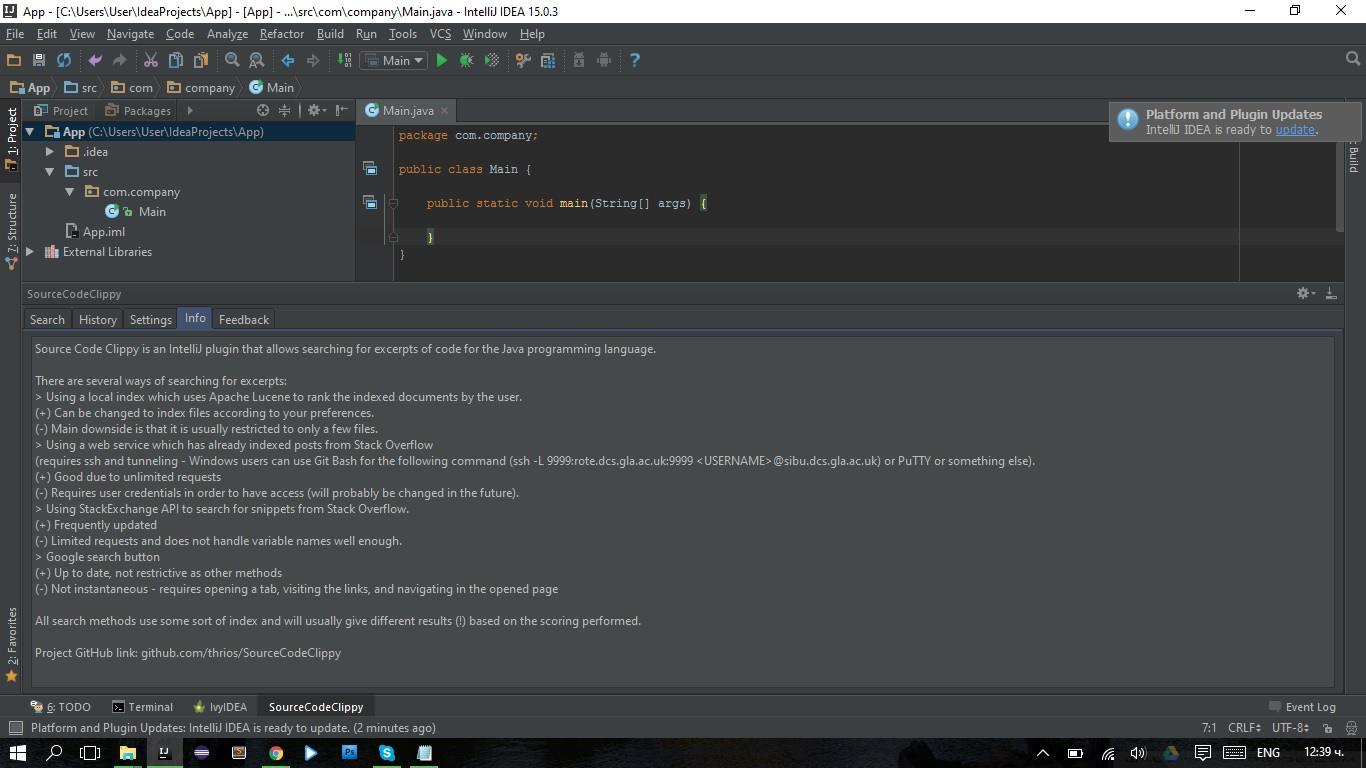
\includegraphics[scale=0.2]{tab-info}
\centering
\label{fig:info-tab}
\end{figure}

\begin{figure}[h]
\caption{Feedback tab, Darcula IntelliJ theme}
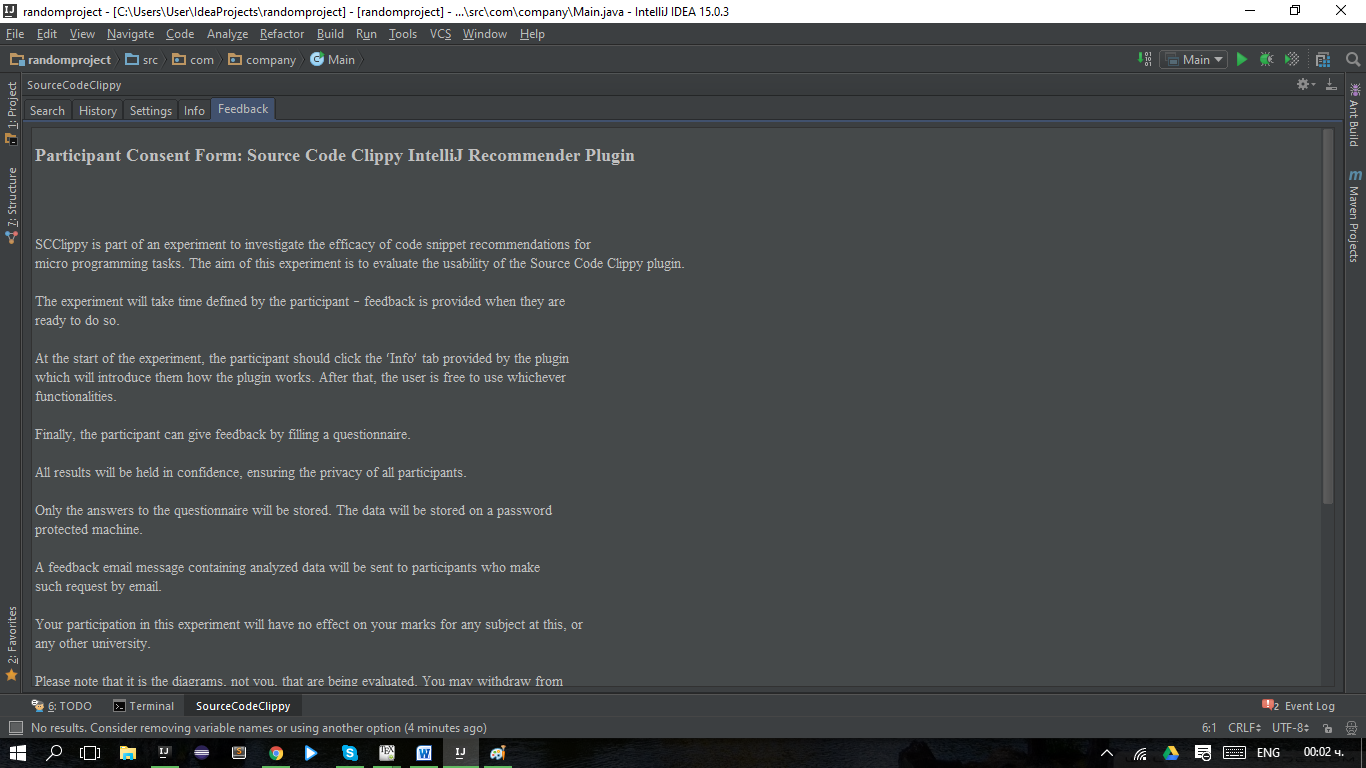
\includegraphics[scale=0.2]{tab-feedback}
\centering
\label{fig:feedback-tab}
\end{figure}

\section{Design decisions}

\textbf{Programming language and IDE choices}\\
Java was the programming language chosen and IntelliJ was picked due to their popularity - Java is frequently used among developers, while IntelliJ is also widely used and in addition offers very useful features to programmers - which were used even when developing the plugin.
\\
\\
\textbf{Java Swing vs Java FX}\\
The plugin's user interface was chosen to be implemented with the Java Swing toolkit rather than Java FX mainly because of familiarity reasons.
\\
\\
\textbf{Searching for excerpts}\\
Searching for code snippets with one method e.g. Stack Exchange API was not enough as it had its limitations and other ways that can provide complementing results existed. Therefore, the system offers a number of techniques for searching excerpts that have been outlined below:

- \textbf{Local index} - offers the user to freely create/update an index on a chosen data set. The major benefit of this approach is that the user can use it while being offline. The downside is that it requires documents, which the user might need, but does not have on their machine - if the user requires more information, about a topic, they may likely not have it.  

- \textbf{Web Service} - has an already indexed collection of Stack Overflow posts for the Java programming language.  The benefit of the web service is that it covers a large dataset - about 2 million documents. In addition, it offers unlimited requests. The negative side is that it is not kept up to date like the Stack Exchange API. 
\\
\\
This method required creating a custom server that provides a RESTful Web Service that on requests performs search using Apache Lucene and returns only the number of documents specified (default is 5) that contain the id, body and score for each post. 
Initially, the server used Lucene to index the extracted files, however a decision was made to make the server use an index on the given PostgreSQL. This approach minimizes the steps needed to index the required posts.
\\
\\
The web service was deployed to an application server (rote.dcs.gla.ac.uk). The major downside is that the it is only available to certain users which need to tunnel to the University's network and login with their credentials in order to have access. The server could have been deployed in the cloud to overcome this problem. However, different providers provide different solutions. For example, some of them do not offer PostgreSQL database support. Deploying the system itself has its own challenges - ideally, it should be done with minimal change of code. The plugin does not feature integration with cloud services. 

- \textbf{Stack Exchange excerpts API} (link) - provides up to date Stack Overflow snippets, but each user has a limited number of requests, equal to 300 daily (by default). Another downside is that it is dependant on variable names e.g. if the user chooses to search for a random string

\textbf{String hsaudhqwudhyqgwd = "";}

then most likely they will not get any results back.

- \textbf{Google Search} - opens a browser tab that searches using the index created by Google on the Stack Overflow's domain. This is a generally good option since it is not so variable independent as the previous type of search.
\\
\\
All of the above methods use an index to process requests quickly and make the plugin more usable. Since they use a different ranking mechanism, the result they return when queried will be different from the others.
\\
\\
\textbf{Automation of features}\\
- \textbf{Querying} - options include:

- Standard way - using a simple button

- Automatic search listener which listens for any activity (typing, deleting or pasting text) which saves time – one less click per query - and is more intuitive.

- Search on 'Enter' key pressed (faster than a button, slower than automatic search). Performed only when the user presses 'Enter'. It is faster than using a button, but slower than automatic search. Although automatic search seems the best, in practice, this option was implemented so as to avoid too many requests as there is a limit on the requests that can be made to Stack Overflow, and to avoid sending too many requests to the web service as they will not be handled at a sufficient pace.
\\
\\
- \textbf{Typing} - when typing the input field is set to contain the text being typed. The text that is captured is triggered on special characters and the text of the last command range is restricted to the last seen semi colon or brace. This way only the relevant text being typed is considered and the approach also prevents ranges of text starting from import statements. The method does not restrict the user to use selection if they wish to capture a bigger piece of code.  
\\
\\
- \textbf{Code Insertion to query pane} - can be done in multiple ways:

- Standard copy paste

- When selecting text the user could right click and select an option to allow him to set the text of the query (search begins automatically) 

- Instant copy paste on highlight
The final options was chosen due to better usability and efficiency.

\textbf{Post size}\\
Currently, posts of all sizes are displayed. The size of posts could have a fixed number of rows and an added scroll. However, the latter idea was not regarded as a particularly good option. If the row number is low, the user would have to scroll. The problem with that is if the result is a single line long, then there would be empty space - a check for query size may be added to avoid that, but there is not much benefit in doing that. It is also more complex. The initial idea does not have drawbacks, therefore, it was implemented.

\textbf{Post content}\\
Since the input from the data sources is often in HTML, each post enables the rendering of HTML (v3.2). The implementation is done through JEditorPane. Originally JTextPane was used, however as it did not offer a lot of customization, it was  turned down. The usage of external libraries are another choice but in this case they were unnecessary.

Posts feature additional statistics - the score of the post, its type (question or answer) and the URI link.

\textbf{Indexing vs Full-Text Search}\\
Indexing was regarded as more suitable than Full-Text search to do the task of retrieving code snippets. The main reason is that indexing platforms are more efficient and flexible - they offer more customization and retrieval is done much faster.

\textbf{Lucene vs Terrier}\\
The choice of an open source indexing platform came down mainly from easiness of implementation. Terrier did not have a proper straightforward tutorial showing a programmatic way of calling the API. Thus, Apache Lucene Core (https://lucene.apache.org/core/) was used for indexing and retrieval of files. Both retrieval platforms have different underlying principles by default (links), however, it should be pointed out that the decision made does mean a less capable system was used.

\textbf{Lucene settings}\\
Stopwords were removed as most code is filtered out due to insufficient length

No stemming is applied since retrieval is fast and there is no need to make the underlying dictionary small and sacrifice details. In terms of precision, the effectiveness of stemming were not compared to those without stemming. 

Special characters are escaped when querying to enable braces and other useful symbols 

Default settings for ranking were used (link):

- Frequent terms in a document increase the documents score
- Popular terms have lower score
- More terms that match the query means higher score
- Short documents over long documents


\textbf{Displaying more results for a query}\\
Additional search request is made (if necessary) when the scroll reaches the bottom of the plugin's tool window. Other options to be considered are: having a button instead (has to be clicked every time, less interactive); making search infinite (not very practical since only the top results are mostly being looked at).

\textbf{IntelliJ notifications} are used to inform the user with feedback. Examples include "Check connection to server. ..." which is displayed when the user is not connected to the Internet or other connection problems have occurred.

\textbf{IntelliJ themes}
The plugin provides the user with the option to change the colour of the text in posts. This is done so that the plugin is not strictly dependent on the theme used by the user. In addition, it enables the them to choose to configure the look of the plugin to match their subjective preferences.

\section{Final design features}
The plugin has its own closable window (ToolWindow) in IntelliJ that features five tabs.

The first tab is for searching. It contains four different types of search for excerpts - one for Google search with the domain of Stack Overflow (clickable by a button) and the rest three are selectable by a combo box:

- Local index

- Web service (uses indexed collection of Stack Overflow Java documents)

- Stack Exchange excerpts API (v2.2)

The search is performed when 'Enter' is typed on the content of an input field which the user can use to write a query. The input field can be used directly, as well as by selecting a code in the current project. The content is also automatically modified by capturing the user's types statements.

More results are also displayed when the scroll reaches the bottom - search is triggered if necessary.

The output of a query comes in forms of posts in the tool window each of
which contains posts from Stack Overflow. The code is highlighted based on code tags.

Along with the content, each post also displays a number of features in the bottom of the post:
The score\\
Type of post (question or answer)\\
The link to the Stack Overflow article is included (or the path to the file if local index is used)\\

For local index and web service search, formatted code insertion can be performed by double clicking on a code snippet in a post - if there are more than one code snippets in a post, the user will be prompt to choose which one.

When searching with Stack Exchange API, the number of calls left are displayed.

The default sorting used is by relevance for all search methods, however, the user could change to see the gathered results sorted by score.

A filter for results can be done by typing a number into a text box that will show only the posts with the minimum number of votes specified.

The plugin offers a feature to go to Stack Overflow to ask a question in case the answer was not found.

The second tab is the search 'History' tab, which enables the user to see recent query searches. Each new entry is displayed at the top.

The third tab is the 'Settings' tab that allows configuring the plugin. The options include:
- General settings\\
> "Auto-resizable query input text area" (checkbox) - offers dynamically resizable query input area or static one that is long 5 rows and uses a scroll\\
> "Highlighted results" (checkbox) - can turn on/off highlighting of results\\
> "Total number of posts" (number pane) - the number of posts after basic search using 'Enter' key \\
> "Total number of posts after scroling down search" (number pane) - controls the number of posts after extended search activated when scrolling to the bottom\\
> "Colour of text" - text colour in posts chosen by typing its name or hex number (see HTML blabla)\\
- Web service options\\
> "Web service URI" (key input pane) - for setting the URI to the chosen service\\
- Local index options\\
> "Current index folder" - path to the index directory for local search\\
> "Create/Update local index" - creates or updates an index by specifying index directory, data directory, and which of the two options.\\

Fourth tab is for plugin information which explains some details of the plugin.

Fifth tab contains the participant consent form and is used to submit feedback by completing an online survey.

\section{Challenges}
- Using Terrier was initially planned for indexing and querying (http://terrier.org/), however, due to the lack of examples and information on how to use its API programmatically, the use of Lucene was considered and used instead.

\chapter{Evaluation}
As already seen, the users can participate in the evaluation of the plugin by going through the following steps:

1. Installing the plugin from IntelliJ (plugin was deployed to the JetBrains plugin repository)

2. Using the plugin's features for a desired period of time

3. Clicking on 'Feedback' tab

4. Reading the participant consent form

5. Clicking on a button, which will open the browser and take them to a survey

6. Answering at least all mandatory questions in the survey, and possibly even optional ones as well

7. Submitting the survey

\section{Unit Testing}
The main functionality of the code was tested using JUnit.

\section{User evaluation (Acceptance testing) and ethics checklist}

\chapter{Conclusion}

\section{Project outcome}

Source Code Clippy is a configurable plugin that enables the search of excerpts from different sources, along with other helpful functionalities.

The plugin was successfully implemented, tested, deployed and evaluated. All requirements were fulfilled, except one 'would-have' responsible for making search more sophisticated - adding tags and/or assigning less weight to variable names as they typically tend to be more irrelevant for a given query.

The evaluation showed that SOMETHING FROM EVALUATION @@@@@@@@@@@@@@@@.

\section{Future work}
It is reasonable to say that the plugin could benefit from having a more intelligent search which can be done using various techniques:

- More weight could be assigned to keywords and relevant code so that less important code such as variable names are not regarded as significant. 

- Making use of tags could prove to be beneficial by matching the user's needs - specifically when they would like to get results only from a subset of the data. Tags can be included for all three types of search (local index, web service, Stack Exchange API).

- Extracting other information from the provided database could help to include more data when returning results or for filtering purposes. For example, one or more of the following columns could be taken into account: 'creationdate', 'viewcount', 'answercount', 'commentcount', 'favouritecount'. The Stack Exchange excerpts API can also be used to its full potential. (http://api.stackexchange.com/docs/)

The plugin can be extended to have:

- Support for multiple languages

- Caching results (not much benefit since retrieval is fast)

- Storing search history permanently

- Options for better interaction with Stack Exchange - login/logout, notification when someone has answered the user's question

\section{Learning outcomes}

At the beginning of this project, there was a lack of experience on how to build an IntelliJ plugin and insufficient knowledge about information retrieval along with its according available platforms. However, by going through the process of creating the plugin, the required skills were learned. In addition, the existing skills of developing software were enhanced by making decisions about ideas and their implementation in practice.

\chapter{Bibliography}

%\vspace{-7mm}
\begin{figure}
\centering
%\includegraphics[height=9.2cm,width=13.2cm]{uroboros.pdf}
\vspace{-30mm}
\caption{An alternative hierarchy of the algorithms.}
\label{uroborus}
\end{figure}

The quick brown fox jumped over the lazy dog.

%%%%%%%%%%%%%%%%
%              %
%  APPENDICES  %
%              %
%%%%%%%%%%%%%%%%
\begin{appendices}

\chapter{Chapter name}
\begin{verbatim}
\end{verbatim}

\end{appendices}

%%%%%%%%%%%%%%%%%%%%
%   BIBLIOGRAPHY   %
%%%%%%%%%%%%%%%%%%%%

\bibliographystyle{plain}
\bibliography{bib}

\end{document}
